\section{Funções Trigonométricas}
\begin{frame}
\frametitle{O Círculo Trigonométrico} 

A relação fundamental $\sen^2 \widehat B + \cos^2 \widehat B = 1$
sugere que os pontos do plano cartesiano $\paren{\cos \widehat B,
\sen \widehat B}$ pertencem a uma circunferência de raio 1, como
mostra a figura abaixo.
\begin{center}
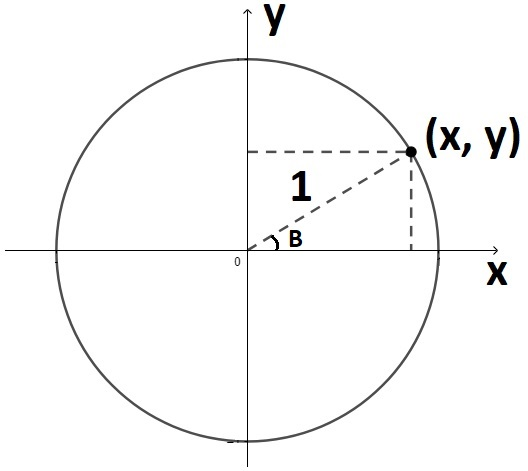
\includegraphics[width=4.5cm]{figures/circtrigB.jpg}
\end{center}

Dessa forma, sendo $\widehat B$ o ângulo medido a partir do eixo
positivo de $x$ e tomando o sentido anti-horário como sentido
positivo, os pontos $(x, y)$ do círculo acima são tais que $x = \cos
\widehat B$ e $y = \sen \widehat B$.


\end{frame}



%------------------------------------------------------------------------------------------------------------

\begin{frame}
\frametitle{O Círculo Trigonométrico} 

Agora, a fim de definirmos as funções trigonométricas como funções
reais, considere a seguinte função, chamada de função de Euler: $E:
\R \to \R^2$ tal que $E(t)$ é o ponto $(x, y)$ do círculo
trigonométrico obtido após ``enrolarmos'', com corda de comprimento
$t$, o círculo trigonométrico iniciando no ponto $(1, 0)$ e tomando
como sentido positivo o sentido anti-horário.
\begin{center}
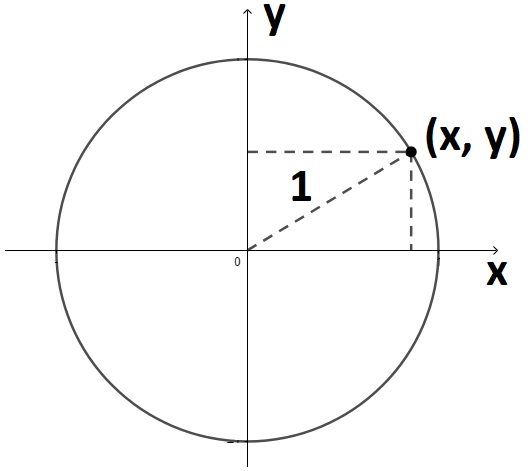
\includegraphics[width=5cm]{figures/circtrig.jpg}
\end{center}
\end{frame}



%------------------------------------------------------------------------------------------------------------

\begin{frame}
\frametitle{O Círculo Trigonométrico} 

\begin{definicao}
As funções $\cos : \R \to \R$ e $\sen : \R \to \R$, chamadas
\sub{função cosseno} e \sub{função seno} respectivamente, são
definidas pondo-se, para cada $t \in \R$,
$$E(t) = \paren{\cos t , \sen t}.$$
\end{definicao}
Em outras palavras, $x= \cos t$ e $y = \sen t$ são, respectivamente,
a abcissa e a ordenada do ponto $E(t)$ da circunferência unitária.

\end{frame}



%------------------------------------------------------------------------------------------------------------